\chapter{Physics Objects}

\label{ch:objects}

\par This chapter introduces the ``physics objects'' used in this thesis in the reconstruction of events. The reconstruction of primary vertices is described in Section~\ref{sec:pv}. 
The reconstruction of electrons, muons and taus is described in Section~\ref{sec:el}, ~\ref{sec:mu} and ~\ref{sec:taus}.
Different types of jets that are used by this analysis in different kinematic regions are described in Section~\ref{sec:jets}. 
The reconstruction of missing transverse momentum (\met) and missing transverse momentum significance, is discussed in Section~\ref{sec:met}. 
Finally Higgs tagging is described in detail in Section~\ref{sec:higgs}.

\section{Inner Detector Tracks and Primary Vertex}
\label{sec:pv}

\par The tracks in the inner detector are based on fitting a trajectory model to a set of measurements using a sequence of algorithms\cite{Cornelissen:1020106}.
\par The inside-out algorithm is the baseline algorithm and is designed for efficient reconstruction of primary particles. 
It starts with three-point seeds in the silicon detectors and adds hits moving away from the interaction point using a combinatorial Kalman filter 
and tracks are extended into the TRT.
\par Then reconstruction of secondary particles produced by the interactions of the primary particles is achieved by back-tracking. 
Back-tracking means the track search starts from segments reconstructed in the TRT and extends inwards by adding silicon hits. 
TRT-standalone tracks refer to tracks from TRT segment without extension into the silicon detectors.					
\par The transverse and longitudinal impact parameters of a track are referred to as $d_0$ and $z_0$ and their resolutions as $\sigma_{d_0}$ 
and $\sigma_{z_0}$. 
\par Each beam crossing generates multiple proton-proton interactions, leading to multiple track vertices reconstructed from the available inner detector tracks.
\par All vertices with at least two associated tracks are retained as valid primary vertex candidates. 
The output of the vertex reconstruction algorithm is a set of three dimensional vertex positions and their covariance matrices, i.e. the vertex corresponding to the hard scatter that generated the physics objects of interest, is selected as the one with the largest $\sum p_T^2$, where the sum is over all associated tracks. 
The basic track selection criteria are summarized in Table~\ref{tab:pv}.

\begin{table}[tbh]
    \centering
    \scriptsize
    \begin{tabular}{|l|c|c}
        \hline
        Aim & Selection \\
        \hline
        Reject soft fake tracks &$p_T> 0.4~GeV$ \\
        \hline
        In ID fiducial volume &$|\eta| < 2.5$ \\
        \hline
        Enough hits for track reconstruction & More than 9 hits between the Pixel\&SCT detectors for $|\eta|\le 1.65$ \\
        \hline
        Enough hits for track reconstruction & More than 11 hits between the Pixel\&SCT detectors for $|\eta|\ge 1.65$ \\
        \hline
        Good hit quality & Less than 2 hits in a SCT detector layer shared by multiple tracks \\
        \hline
        Good hit quality & Less than 1 hits in a Pixel detector layer shared by multiple tracks \\
        \hline
        Good hit quality & 0 missing hit in the Pixel detector when a hit is expected \\
        \hline
        Good hit quality & Less than 1 missing hits in the SCT detector when hits are expected \\
        \hline
    \end{tabular}
    \caption{Selection criteria for tracks used in the reconstruction of to reconstruct vertices.}
    \label{tab:pv}
\end{table}

\section{Electrons}
\label{sec:el}

\par Electron candidates are clusters of energy associated with ID tracks, 
where the final track-cluster matching is performed after the tracks have been fitted with a Gaussian-sum filter.
\par A few variables are checked to identify electrons while suppressing background objects 
such as hadronic jets or converted photons~\cite{ATL-PHYS-PUB-2015-041}. 
They are the hits in the silicon detectors, including a hit in the IBL, and a likelihood discriminator, 
which combines the shower shape information provided by the highly segmented calorimeter, high-threshold hits in the TRT, 
compatibility of the tracking and calorimeter information, track quality information, 
as well as the impact parameter in the transverse plane ($|d_0|$) and its significance ($\frac{|d_0|}{\sigma_{d_0}}$).
\par Electron isolation measures the detector activity around an electron candidate, 
and can be used to further reject backgrounds such as electrons originating from converted photons produced in hadron decays, 
electrons from heavy flavor hadron decays, and light hadrons misidentified as electrons.
\par There are several working points of the likelihood variable corresponding to the strictness of requirements imposed on electrons. 
This analysis uses the LooseLLHBLayer working point. 
In addition, two types of electrons are selected in this analysis: VHLoose and ZHSignal. The definitions of VHLoose and ZHSignal electrons are summarized in Table~\ref{tab:el}.

\begin{table}[tbh]
    \centering
    \begin{tabular}{|l|c|c|c|c|c|c|c}
        \hline
        Electron Type & $|p_T|$ & $|\eta|$ & $\frac{|d_0|}{\sigma_{d_0}}$ & $z_0\dot sin\theta$ & Likelihood & Isolation \\
        \hline
        VHLoose &$>7$&$<2.47$&$<5$&$<0.5$&LooseLLHBLayer&LooseTrackOnly \\
        \hline
        ZHSignal&$>27$&$<2.47$&$<5$&$<0.5$&LooseLLHBLayer&LooseTrackOnly \\
        \hline
    \end{tabular}
    \caption{Definitions for the different categories of electron.}
    \label{tab:el}
\end{table}

\par The VHLoose definition is used in the Signal Region whereas the ZHSignal definition is used in some control regions.
 
\section{Muons}
\label{sec:mu}

\par Muon reconstruction is performed based on information from the inner detector, muon spectrometer and calorimeters. Explained in~\cite{Aad:2016jkr}, there are five types depending on different reconstruction methods.

\begin{itemize}
    \item Combined muons are reconstructed by combining the hits of the ID track and MS track and the energy loss in the calorimeter.
    \item Segment-tagged muons are formed from a track in the ID if it is associated with at least one track segment in the MDT or CSC chambers. It captures muons passing only one layer of MS chambers, due to their low \pt~or reduced MS acceptance in the region.
    \item Extrapolated muons are reconstructed based only on the MS track and a loose requirement on compatibility with originating from the IP. They are used to extend the acceptance for muon reconstruction into the region $2.5 <\eta< 2.7$, where three layers are required.
    \item Calorimeter-tagged muons. In the region of $|\eta< 0.1$, ID tracks with $15 ~GeV < p_T < 100 ~GeV$ are identified as muons if their energy deposits in the calorimeter match that expected from minimum ionizing particles. They recover muon acceptance in the region where the MS is only partially instrumented.
\end{itemize}

\par Similar to Electron reconstruction, there are different muon identification working points. This analysis choeses ``Loose'', defined as muons reconstructed using any reconstruction methods, and ``Medium'', reconstructed using either the Combined muon or Extrapolated muon methods. The VHLoose definition is used in the signal region whereas the ZHSignal definition is used in some control regions.					
\par As shown in Table~\ref{tab:mu}, this analysis applies additional criteria to muons in different regions. A tighter selection is required in control regions for a high muon purity and a looser selection when muons are not desired and are vetoed in the signal region.

\begin{table}[tbh]
    \centering
    \begin{tabular}{|l|c|c|c|c|c|c|c}
        \hline
        Electron Type & $|p_T|$ &$|\eta|$ & $\frac{|d_0|}{\sigma_{d_0}}$&$z_0 sin\theta$ & Likelihood &Isolation \\
        \hline
        VHLoose &$>7$&$<2.7$&$<3$&$<0.5$&Loose&LooseTrackOnly\\
        \hline
        WHSignal &$>25$&$<2.5$&$<3$&$<0.5$&Medium&FixedTrackTTTight\\
        \hline
        ZHSignal &$>25$&$<2.5$&$<3$&$<0.5$&Loose&LooseTrackOnly\\
        \hline
    \end{tabular}
    \caption{Definitions for the different categories of muons.}
    \label{tab:mu}
\end{table}

\section{Taus}
\label{sec:taus}

% Tau, what and why
\par The Tau lepton, unlike the lighter leptons, electron and muon, 
is the only lepton that can decay hadronically. The branching ratio to hadrons is 64.79\%. Therefore, it is important to reject events with hadronically decaying tau lepton.

% How to reject tau with Loose Tau ID
\par Hadronicallly decaying tau leptons can be reconstructed as small-radius jets and identified with a tree-based machine learning algorithm. A typical tau jet 
contains either one or three charged hadrons, which can be exploited in the tree-based classifiers to differentiate from QCD jets. With the trade-off of selection 
efficiencies and fake rate, three classifiers, loose, medium, tight, can be determined. More details can be found in Ref\cite{ATL-PHYS-PUB-2015-045}. 
In order to suppress the tau background to a maximum extent, the loose working point is chosen to build the tau veto condition, together with the baseline section of $p_T > 25 GeV$ and $|\eta| < 2.5$.

\section{Jets}
\label{sec:jets}

\par In proton-proton collisions, almost immediately after being produced, a quark or gluon fragments and hadronizes, leading to a collimated spray of energetic hadrons -- 
a jet~\cite{Salam:2009jx}. There exist many different jet clustering algorithms to measure the jet properties. 
\par Among all jet finding algorithms, the anti-$k_T$ algorithm~\cite{Cacciari:2008gn} is now most commonly used. This algorithm favors clusterings that involve hard particles, 
and the jets then grow outwards around hard ``seeds''. The radius R represents the clustering distance metric. It determines the radial size of the jet in the $\eta-\phi$ plane.

\par Calorimeter jets are reconstructed by combining topological clusters of energy deposits in the calorimeter~\cite{Aad:2011he}, while the inputs to track jet clustering are inner detector (ID) tracks. 
Small-radius (R=0.4) calorimeter jets are designed to capture the four-momentum of a single hard quark or gluon produced in the pp collision. For jets that are from collimated decay products of heavy particles or low \pt~jets, 
a large cone size is used to contain all of the decay products. Large-radius jets are defined as calorimeter jets reconstructed with the anti-$k_T$ algorithm with R = 1.0. 
The large-radius calorimeter jets are used for Higgs boson reconstruction in the boosted topology in this analysis.

\par In this iteration of the analysis, variable radius track jets used for b-quark identification inside the large-radius jets.

\subsection{Calorimeter jets}
\label{sec:calo}

\par Topological clusters (topo-clusters) that are cells are clustered together to reconstruct particle showers, exploiting the fine granularity of the calorimeters. 
The topo-cluster reconstruction is based on cell signal significance S/N, defined as the ratio of cell energy at electromagnetic energy scale over average expected noise. 
The reconstruction starts from a seed cell with signal significance above the threshold of S/N = 4. Then the neighbouring cells with signal significance over S/N = 2 are included iteratively. 
Finally, all calorimeter cells neighbouring the formed topo-cluster are added.

\begin{figure}[htbp]
    \centering
    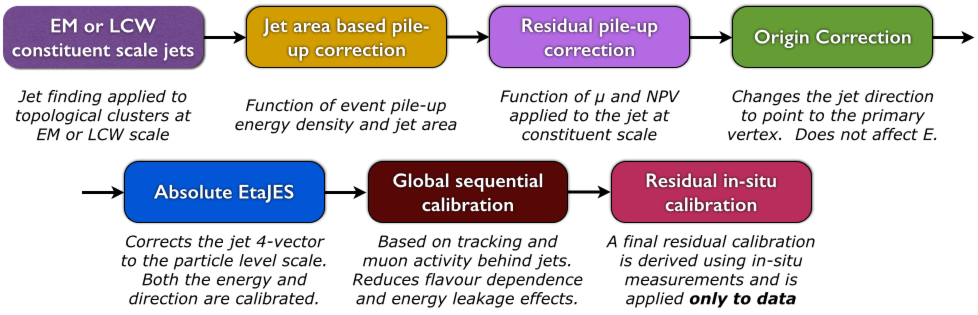
\includegraphics[width=1\textwidth]{chapters/c5/figures/jet_calib}
    \caption{Calibration stages for reconstructed jets.}
    \label{fig:jet-calib}
\end{figure}

\par After jets are reconstructed, a calibration is applied to the jet four momentum of to recover the particle-level energy scale.
A series of calibrations are applied after jet clustering as shown in Fig~\ref{fig:jet-calib}.

\begin{itemize}
    \item \textbf{Jet area-based pile-up correction} This step are designed to remove the excess energy from pile-up interactions. The area-based \pt~density subtraction is applied event-by-event~\cite{Cacciari:2007fd}. The \pt~density is estimated using the medium of \pt~density of all jets in the event calculated by \pt/A, where A is the jet area.
    \item \textbf{Residual pile-up correction} A residual \pt~dependence on in-time pile-up evaluated through the number of reconstructed primary vertices and out-of-time pile-up $\mu$ is roughly linear. So a linear correction is applied with coefficients derived from MC simulation. 
    \item \textbf{Origin correction} The kinematic observables of each topo-cluster are recalculated using the vector from the primary hard-scattering vertex to the topo-cluster centroid as its direction. The resolution of $\eta$ can be improved in this step. The jet energy is unaffected.
    \item \textbf{Absolute MC-based calibration} An absolute jet energy and $\eta$ correction is derived from MC simulation. The average energy response is defined as the mean of $E_{reco}/E_{truth}$ binned in $E_{truth}$ and $\eta_{jet}$. A similar correction is done for $\eta$.
    \item \textbf{Global sequential calibration} The global sequential calibration (GSC) method~\cite{Aad:2011he} is applied to improve resolution of the Jet Energy Scale (JES) resolution. In this step, JES depends on five features which account for different aspects and the calibration factor is derived from MC. The procedure is similar to the absolute JES calibration.
    \item \textbf{Residual in situ calibration} This steps aims at correcting the difference between data and MC. For jets up to 950 GeV and with $|\eta| < 0.8$, calibration factors are derived from Z+jet and $\eta$+jet balance, while, for high-\pt~jets up to 2 TeV, the multijet balance is used.
\end{itemize}

\par The larger the jet size, the more chances there are that particles from the underlying events, pile-up interactions and soft radiation contaminate the jet. Thus for large R jets, three techniques of jet grooming are developed:
split-filtering~\cite{Butterworth:2008iy}, pruning~\cite{Ellis:2009me} and trimming~\cite{Krohn:2009th}. 

\begin{itemize}
    \item \textbf{Split-filtering} Large-radius jets are rebuilt using the Cambridge/Aachen (C/A) algorithm. C/A jets are then de-clustered by splitting the jet into two pieces into pieces, starting from the last C/A merge. De-clustering continues with the highest mass piece 
    until the requirements on mass-drop $\mu_{12} < \mu_{max}$ and momentum balance $\sqrt{y_{12}} > \sqrt{y_{min}}$ are met. The momentum balance and mass drop are defined as $y_{12} = \frac{min(p_{T1},p_{T2})}{m_{12}}\Delta R_{12} $, $\mu_{12} = max(m_1,m_2) m_{12}$, where $m_{12}$ 
    is the invariant mass of two pieces. If the requirements are not satisfied, the jet is discarded. Filtering aims at removing soft radiations that is irrelevant to the hard scattering process. 
    In the filtering stage, constituents of the surviving jet are reclustered with subjet size $R_{sub} = min(0.3,\Delta R_{12})$, where $\Delta R_{12}$ is taken from the splitting stage.
    \item \textbf{Trimming} Large-R jets are reclustered using the $k_T$ algorithm, 
    which favors clustering low \pt~constituents first. This creates a set of subjets with radius parameter $R_{sub}$. 
    Subjets with an energy below some threshold fraction of the energy of the large-radius jet are removed from the large R jet.
    \item \textbf{Pruning} Pruning is similar to trimming as it removes constituents with relative small $p_T$, while it has an additional wide-angle radiation veto. 
    Constituents of ungroomed large-radius jet are then re-clustered with the C/A algorithm. In each pairwise clustering step, secondary constituents with wide-angle 
    $\Delta R_{12} > R_{cut} \times \frac{2M}{p_T}$ or soft property are discarded. The definition of being soft is that $f_2 < Z_{cut}$ where $f_2$ is the fraction of the softer constituent \pt~with respect to the pair.
\end{itemize}

\par Trimmed large-radius jets are used to reconstruct Higgs candidates when the b-quark decay products of the Higgs are too collimated to resolve by two small-radius jets.

\par Small-radius jets used in the analysis can be divided into two categories: central jets and forward jets. Forward jets are small-radius jets with $2.5 < |\eta| < 4.5$ and $p_T > 30 GeV$, and can be used to reduce backgrounds. 
Small-radius jets with $|\eta| < 2.5$ and \pt~$> 20 GeV$ are called central jets and they are used to reconstruct Higgs candidates with low or moderate \pt~.
For central jets with $|\eta| < 2.4$ and $20 GeV < p_T < 60 GeV$, an additional requirement on the jet vertex tagger value $JVT > 0.59$ is imposed. Details on the jet vertex tagger (JVT) can be found in Ref~\cite{Aad:2015ina}.

\subsection{Track jets}
\label{sec:track}

\par Track jets are jets built entirely from tracks reconstructed in the inner detector. In Run 2, track jet b-tagging became the standard approach to resolve the heavy flavor components from boosted decay of heavy resonances~\cite{ATL-PHYS-PUB-2015-035,ATLAS-CONF-2016-039}. Studies of track jet calibration can be found in Ref~\cite{VanDenWollenberg:1981533}. 
\par In this thesis, two types of track jets are discussed. R = 0.2 track jets will be referred to as FR track jets, for fixed radius track jets, in contrast to the variable radius (VR) track jets.

\par A track selection of input ID tracks is applied in order to suppress fake tracks and tracks from pile-up vertices. The selection criteria are summarized in Table~\ref{tab:trk}. With a relatively looser requirement on hits in the ID detectors compared to the track selection criteria for primary vertex reconstruction, a small longitudinal impact parameter of the tracks with respect to the primary vertex is required to reject pile-up vertices.

\begin{table}
    \centering
    \scriptsize
    \begin{tabular}{|l|c|c}
        \hline
        Aim & Selection \\
        \hline
        Reject soft fake tracks &$p_T> 0.4 GeV$ \\
        \hline
        In ID fiducial volume &$|\eta| < 2.5$\\
        \hline
        enough hits for track reconstruction & More than 7 hits between the Pixel and SCT detectors \\
        \hline
        good hit quality& Less than 1 hit in a Pixel shared by multiple tracks\\
        \hline
        good hit quality&Less than 1 missing hit in the Pixel detector when a hit is expected\\
        \hline
        good hit quality&Less than 2 missing hits in the SCT detector when hits are expected\\
        \hline
        reject tracks from pile-up & $z_0 \dot sin(\theta) < 3 mm$\\
        \hline
    \end{tabular}
    \caption{Selection criteria for tracks to cluster track jets. }
    \label{tab:trk}
\end{table}

\par FR track jets are then built by applying the anti-$k_T$ algorithm with R = {0.4, 0.3, 0.2} on selected tracks. Track jets in the fiducial region with $p_T > 7 GeV$ and $|\eta| < 2.5$ are accepted as track jets with $p_T < 7 GeV$ are dominated by light jets~\cite{ATL-PHYS-PUB-2014-013}. 				
\par VR track jets are clustered using the anti-$k_t$ algorithm from tracks with the same selection criteria used for R = 0.2 track jets. The main feature of the VR track jet reconstruction~\cite{Krohn:2009zg}, compared to the FR jets is the \pt~dependence of the jet radius:
\begin{equation}
R \rightarrow R_{eff}(p_T) \approx \frac{\rho}{p_T}
\end{equation}
where the parameter $\rho$ shows how the effective jet radius scales with the \pt~of the pseudo-jet during the jet finding procedure, $R_{min}$ and $R_{max}$ are a lower and an upper cut-off on the jet radius.
To optimize the efficiency of double b-tagging over a wide mass range, $\rho = 30 GeV$, $R_{min} = 0.02$ and $R_{max} = 0.4$~\cite{ATL-PHYS-PUB-2017-010}.

\subsection{Ghost Association}
\label{sec:ga}

\par In practice, track jets are seldom used alone for object reconstruction and instead used along with the large-radius calorimeter jets. Calorimeter jets are in charge of providing jet reconstruction while track jets are in charge of providing flavor tagging information. To match track jets to calorimeter jets is the first step for flavor tagging of calorimeter jets. 
\par Ghost association~\cite{Cacciari:2007fd,Cacciari:2008gn} is a method to associate the ``ghosts'' (particles, jets or tracks) to jets by giving them negligible momentum and clustering them within the jets. This is to make sure that the hard-particle content of the jet is unaltered by the addition of the soft ghost particles during jet reclustering. The jet substructure after reclustering is unchanged compared to the previous jet, but with the addition of ``ghosts'' as constituents.
\par An object (track, jet, truth particle) is ghost-associated to a jet if its ``ghost'' is clustered as a constituent of the jet.
\par Compared to $\Delta R$ association which matches objects based on angular distance, ghost association is more robust when dealing with overlapping jets or jets that are not cone-shaped.

\subsection{Flavor tagging}
\label{sec:track}

\par The identification of b-jets is referred to as b-tagging or flavor tagging. After the fragmentation of b-quarks, about 70\% of the b-quark energy goes into the weakly decaying b-hadrons (~5 GeV). With an intrinsic life-time of $1.5 \times 10^{−12}$ s, the average decay lengths for b-hadrons of 30 GeV is about 3 mm, which can be measured with the high-precision tracking system in ATLAS.
The c-hadrons from b-hadrons decay have similar average lifetimes, and thus lead to an additional decay vertex. 
Several b-tagging algorithms are in use to exploit the decay patterns. 				
\par ID tracks are used for these b-tagging algorithms, and tracks need to pass the basic quality cuts. 		
\par These three b-tagging algorithms below are used to provide complementary information and combined using a boosted decision tree (BDT) to provide a score to distinguish between different flavors (c, b, light). 	

\begin{itemize}
    \item \textbf{Impact Parameter Based Algorithms (IP2D and IP3D)} As shown in Fig.2 from Ref~\cite{ATL-PHYS-PUB-2015-022}, tracks from a displaced vertex have larger impact parameter than those coming from the primary vertex. The probability density functions (PDFs) for the signed impact parameter significance of these tracks $\frac{d_0}{\sigma_{d_0}}$ and $\frac{z_0}{\sigma_{z_0}}$ are used to define probability ratios of the jet hypotheses of different flavors, and these are then combined in a single log likelihood ratio discriminant (LLR). While IP2D only uses the transverse impact parameter, IP3D uses the 2D template with correlation between the transverse and longitudinal direction. 
    \par Both IP2D and IP3D assume that all tracks are independent and use naive Bayesian models which ignore correlations between tracks. Besides, while it is easy to build 2D or 3D template histograms, it is technically hard to encode too many variables at the same time. To improve the results, new algorithms which make use of recurrent neural networks with the same input tracks as IP2D/IP3D are developed in ATLAS b-tagging~\cite{ATL-PHYS-PUB-2017-003}.
    \item \textbf{Inclusive secondary vertex reconstruction algorithm (SV)} The secondary vertex based algorithm explicitly reconstructs an inclusive displaced secondary vertex within the jet. Tracks passing quality cuts are first paired to form two-track vertex. These two-track vertices are then be filtered to reject those coming from decays of long-lived particles such as $K_s$, $\Lambda$, photon conversions or hadronic interactions with detector material. An inclusive secondary vertex is fit using surviving tracks using a Kalman filter in an iterative way with certain quality cuts applied.
    \item \textbf{Decay chain multi-vertex reconstruction algorithm (JetFitter)} The decay chain multi-vertex reconstruction algorithm is called JetFitter and exploits the cascade decay structure of b- and c-hadrons to reconstruct the decay chain $Primary\ Vertex \rightarrow b \rightarrow c$ using a Kalman filter. 
    \par Unlike the SV algorithm, the vertex in JetFitter refers to the intersection between tracks and estimated decay chain direction and thus a vertex can have only one track associated to it. Thus JetFitter typically has a much higher reconstruction efficiency, as well as a higher fake rate. To reduce the fake rate, a set of topological variables are built in JetFitter for discrimination purposes. 
\end{itemize}		

\par After running each b-tagging algorithm independently, the output discriminative variables of each algorithm, as well as the kinematic properties of jet \pt~and $\eta$ are combined using a BDT. The \pt~and $\eta$ distributions for signal and backgrounds are re-weighed to match each other before training so that these kinematic variables are not treated as discriminative variables.
\par The training is performed on high purity $t\bar{t}$ and $Z'$ MC samples with at least millions of events. While b-jets are used as signal jets, 
the background is a mixture of c-jets and light-jets. Three versions of the mixture are used: MV2c00, MV2c10 and MV2c20. The number after the character ``MV2c''
shows the percentage of c-jets in the background mixture. Depending on the physics processes, users can choose any of these three version.
The higher the number, the better the discrimination power against c-jets at the cost of reduced light-jet rejection. 
The performance of MV2c10 tagger~\cite{Varni:2655785} for discrimination against light-jet and c-jets can be found in Fig~\ref{fig:mv2c10}.

\begin{figure}[htbp]
    \centering 
    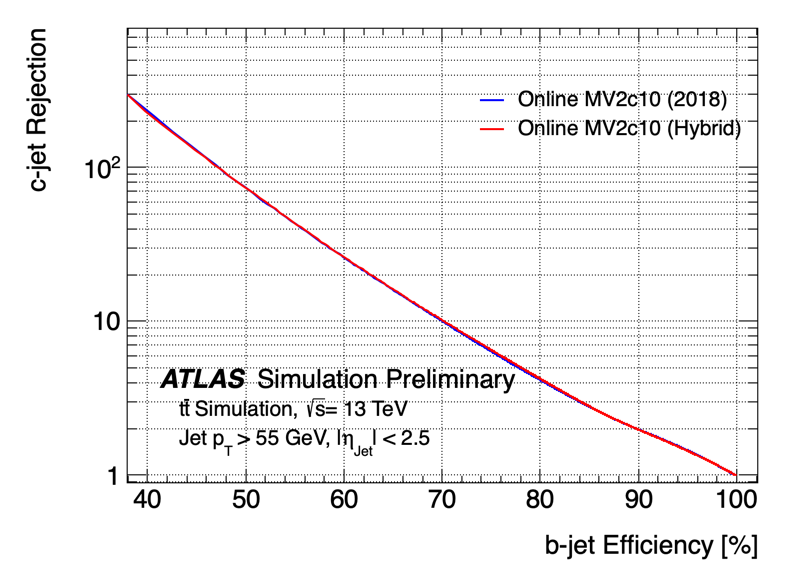
\includegraphics[width=0.4\textwidth]{chapters/c5/figures/ROC_cb}
    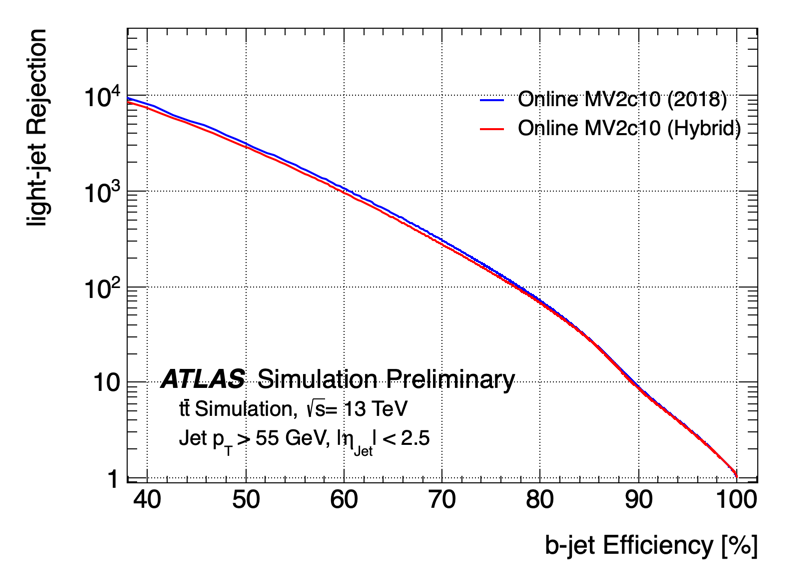
\includegraphics[width=0.4\textwidth]{chapters/c5/figures/ROC_lb}
    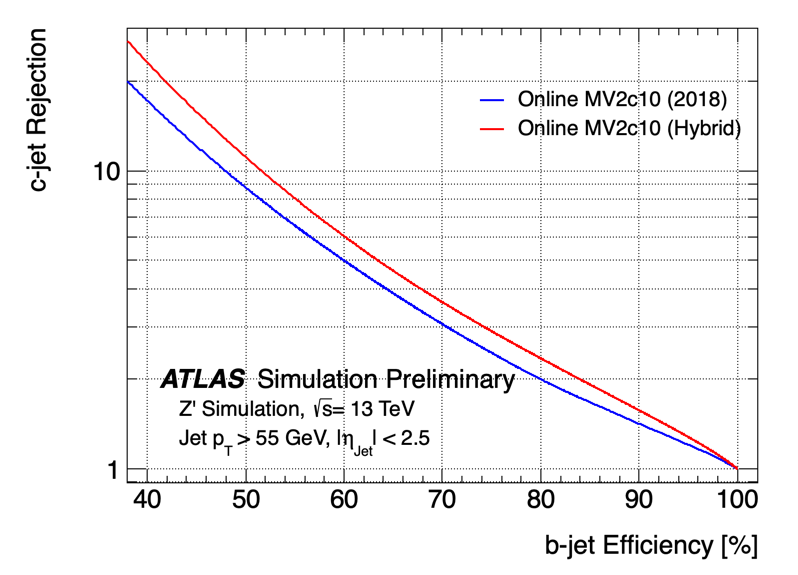
\includegraphics[width=0.4\textwidth]{chapters/c5/figures/ROC_cb_Zprime}
    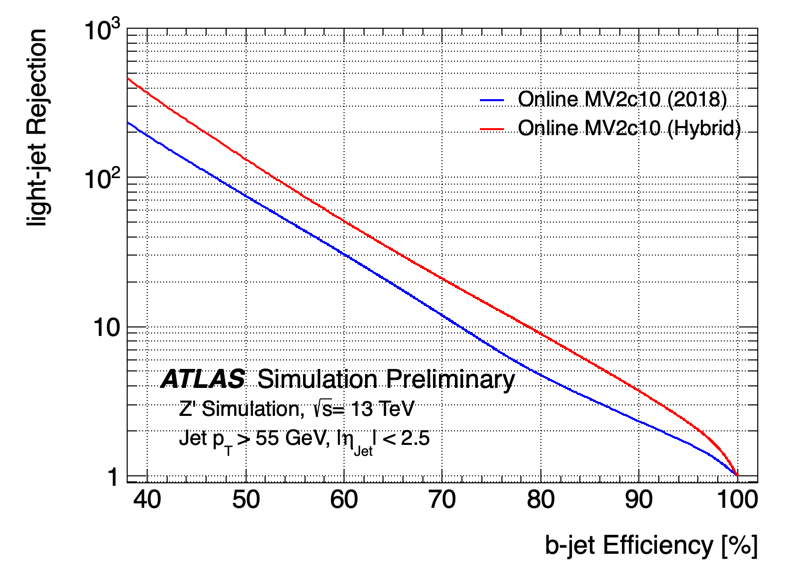
\includegraphics[width=0.4\textwidth]{chapters/c5/figures/ROC_lb_Zprime}
    \caption{The Expected performance of the \textit{b}-tagging algorithm (MV2c10) for \textit{b}-jet triggers in 2018 data-taking (blue solid line) is compared to the same \textit{b}-tagging algorithm trained on the Hybrid training sample (red solid line).}
    \label{fig:mv2c10}
\end{figure}

\section{Missing Transverse Momentum (\met) and Missing Transverse Momentum Significance}
\label{sec:met}

% What is MET
\par According to the conservation of momentum, the sum of the transverse momenta of all particles produced in collisions is zero. Considering the existence of non-detected objects, the transverse momenta from detected objects need not be balanced. The unbalanced part of the transverse momentum is called ``missing transverse momentum''(\met), or MET for short.

% How to calculate MET with/without Tracker fully involved.
\par As mentioned in the last paragraph, the \met~is derived from all detected objects. The \met~calculation is the most difficult object not only because it needs accurate measurement of all detected objects from various detectors, but also of the small fraction of energy deposits that are not clustered by any algorithm. As a result, the \met~scale and \met~resolution are affected by many factors, such as missing muons, mismeasured jets, beam pile-up, etc. In the ATLAS experiment, the \met~reconstruction uses energy deposits in the calorimeters and muon tracks reconstructed in the muon detectors. The Trackers' information is also used to recover the low \pt fraction missed in the calorimeters \cite{ATLAS-CONF-2013-082}. Therefore, both hard objects (high \pt~), like electrons, jets, muons, etc, and soft objects, like track soft terms, are considered in the \met~reconstruction.

% MET significance
\par The uncertainty of \met~calculation result can be large due to the complexity of the reconstruction algorithm. Therefore, a significance variable can be introduced to describe the reliability of the derived \met. The \met~significance is defined as
$$ S=\frac{\met}{\sqrt{\sum_{i}E_{Ti}}}, $$
where the numerator is the amplitude of the derived \met, and the denominator is the scalar sum of the detected objects that are used in reconstructing the \met. A high value of \met~significance suggests the event is more likely to contain an invisible object than be due to resolution smearing.

\section{Higgs tagging}
\label{sec:higgs}

\par For a Higgs particle with sufficiently low \pt, two outcoming b-quarks can be reconstructed individually as small-radius equals to 0.4 calorimeter jets. However, for a Higgs particle with high \pt, 
the two outcoming b-quarks are too collimated to be reconstructed using small-R jets.
``Higgs tagging'' refers to the techniques used to identify boosted Higgs decays to b-quarks. The Higgs candidate is reconstructed as a trimmed large-R jet 
with two ghost-associated b-tagged subjets, reconstructing the b-hadrons.

\subsection{Higgs tagging with advanced subjets}

\par Three techniques are used to tag boosted Higgs bosons: variable-radius track jets (Fig~\ref{fig:vr}), Exclusive-kT (ExKt) and Center-of- Mass (CoM) tagging. These allow to probe the very boosted region~\cite{ATL-PHYS-PUB-2017-010}, where b-hadron decay products are too collimated to resolve even with R = 0.2 track jets.
\par For variable-radius track jets, the parameters $\rho = 30 GeV$, $R_{min} = 0.02$ and $R_{max} = 0.4$ 
are chosen after scanning different $\rho$ and radius as values in Fig.~\ref{fig:vr-scan}. ExKt refers to exclusive regions of interest using exclusive-kT declustering of the large-radius jets. 
CoM jets are constructed via exclusive-kT declusting in the jet's center of mass frame instead of in the lab frame.

\begin{figure}[htbp]
    \centering
    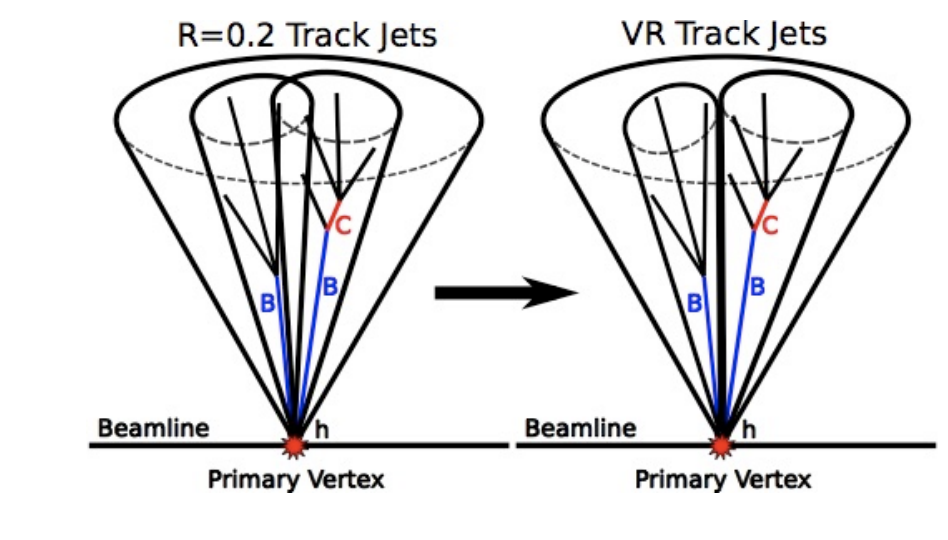
\includegraphics[width=0.6\textwidth]{chapters/c5/figures/VR}
    \caption{A cartoon depicting using VR track jets instead of R = 0.2 track jets.}
    \label{fig:vr}
\end{figure}

\begin{figure}[htbp]
    \centering
    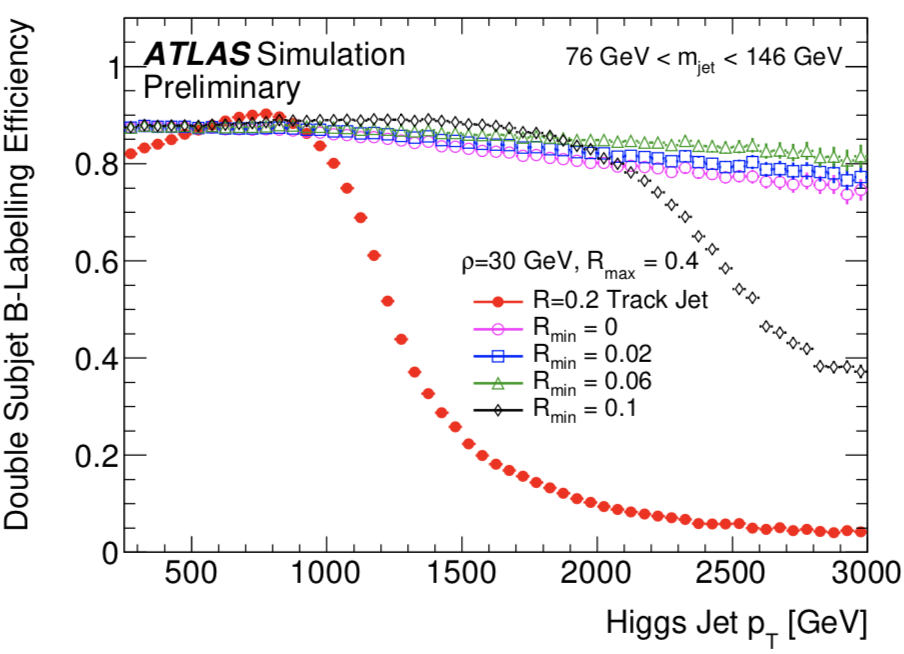
\includegraphics[width=0.4\textwidth]{chapters/c5/figures/r-vr}
    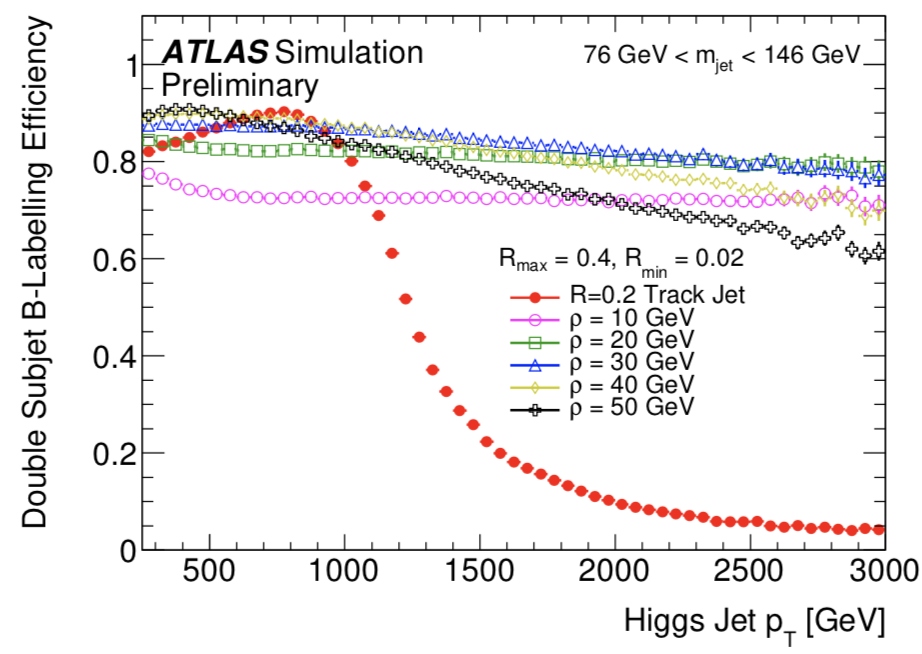
\includegraphics[width=0.4\textwidth]{chapters/c5/figures/rho-vr}
    \caption{Higgs effiency using two VR track jets with different R parameter (Left) and $\rho$ parameter (Right)} 
    \label{fig:vr-scan}
\end{figure}

\par The double b-tag performance for the FR track jet, VR track jet, ExKt and CoM techniques can be found in Fig.~\ref{fig:higgs_pt}.
The plot shows a dramatic decrease for the R = 0.2 track jet technique as the Higgs jet \pt~becomes larger than 1.2 TeV where the 
R = 0.2 track jets are expected to merge. These new techniques, however, can reconstruct Higgs jets with a \pt~of 3 TeV. Receiver operating characteristic (ROC) curves showing Higgs jet tagging performance versus 
QCD jet rejection are shown in Fig.~\ref{fig:higgs_ROC}.

\begin{figure}[htbp]
    \centering
    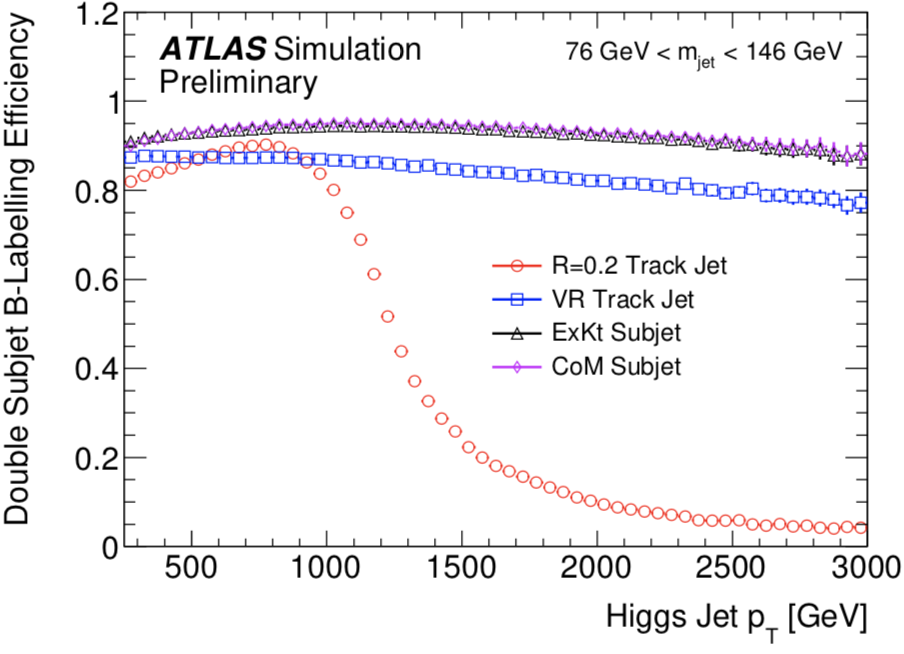
\includegraphics[width=0.6\textwidth]{chapters/c5/figures/higgs_pt}
    \caption{Higgs efficiency using four different subjet techniques: R = 0.2 track jets, VR track jets, ExKt calorimeter jets, and CoM calorimeter jets.}
    \label{fig:higgs_pt}
\end{figure}

\begin{figure}[htbp]
    \centering
    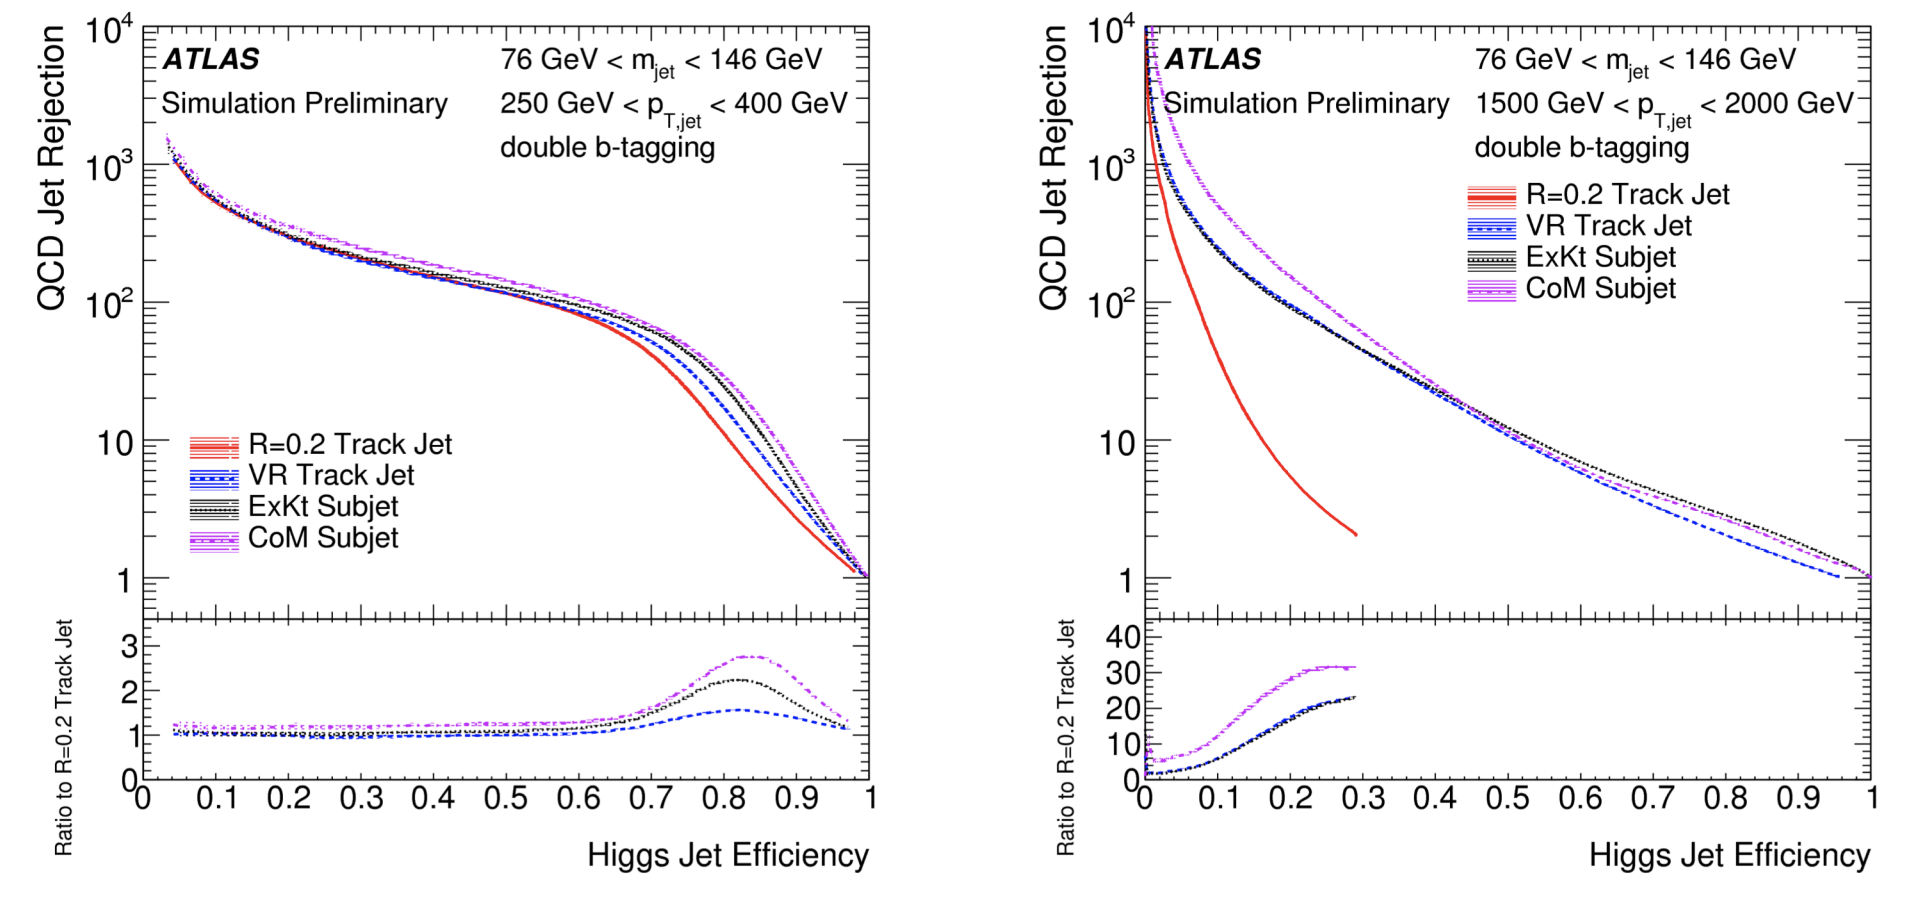
\includegraphics[width=1\textwidth]{chapters/c5/figures/higgs_ROC}
    \caption{ROC curves using four different subjet techniques: R = 0.2 track jets, VR track jets, ExKt calorimeter jets, and CoM calorimeter jets in two different jet \pt ranges}
    \label{fig:higgs_ROC}
\end{figure}

\par The variable-radius track jet technique was chosen to use as subjets in the mono-Higgs analysis as an existing framework to calibrate track jet b-tagging efficiency was readily available in ATLAS.
